\chapter{Metodologías}

El presente capítulo está orientado a describir la manera en que se aplicará las metodologías propuestas en el capítulo anterior y los resultados esperados de los objeticos específicos.

\section{Personal Extreme Programming (PXP)}

Como se mencionó en el Capítulo 2.4.1, la metodología PXP adopta las mejores prácticas de las metodologías Personal Software Process (PSP) y Extreme Programming (XP). Se basa en un desarrollo personal pero a la vez sigue manteniendo las fases claves como Requerimientos, Planififcación e Iteración.

\subsection{Requerimientos }

Durante esta fase, se realiza una entrevista entre el desarrollador y el cliente para capturar los requerimientos iniciales del sistema. Estos requerimientos se transforman en la fase siguiente en historias de usuario, lo que permite enfocar el desarrollo en la experiencia del usuario.

\subsection{Planificación}

Durante esta fase, la actividad central consiste en la creación, priorización y organización de las historias de usuario (HU), las cuales se dividen y asignan a iteraciones específicas. En esta fase también se toman las decisiones de diseño de la aplicación, tales como las configuraciones base de las tecnologías a utilizar, arquitecturas de software y mockups, que permitirán el flujo de las distitnas vistas que tendrá la aplicación y su interacción con los usuarios.

\tituloparpegado{Historias de usuario}
A continuación, la Tabla \ref{tab:hu} ilustra las historias de usuario obtenidas a partir de la entrevista inicial con el cliente.

\begin{longtable}{|l|p{3.5cm}|p{9.5cm}|}
  \caption{Historias de Usuario} \label{tab:hu}\\
  \hline
  \textbf{HU} & \textbf{Actor(es)} & \textbf{Descripción} \\
  \hline
  \endfirsthead
  \multicolumn{3}{c}{\textbf{\tablename\ \thetable{} -- Continuación de la página anterior}} \\
  \hline
  \textbf{HU} & \textbf{Actor(es)} & \textbf{Descripción} \\
  \hline
  \endhead
  \hline
  \multicolumn{3}{|r|}{Continúa en la siguiente página...} \\
  \hline
  \endfoot
  \hline
  \endlastfoot
  HU01 & Tatuador & quiero registrarme en la plataforma ingresando mis datos, para tener un espacio de trabajo integral. \\ \hline
  HU02 & Tatuador & quiero iniciar y cerrar sesión mediante mis credenciales, para proteger la privacidad de mi negocio. \\ \hline
  HU03 & Tatuador & quiero recuperar mi contraseña en caso de olvido, para no perder el acceso a mi agenda e inventario. \\ \hline
  HU04 & Tatuador & quiero importar imágenes a la plataforma, para almacenarlas en la nube. \\ \hline
  HU05 & Tatuador & quiero ver todos mis diseños en una galería, para acceder a ellas de manera expedita. \\ \hline
  HU06 & Tatuador & quiero eliminar un boceto antiguo de la galería, para mantener mi espacio ordenado y liberar almacenamiento. \\ \hline
  HU07 & Tatuador & quiero añadir etiquetas a mis bocetos, para filtrarlos y encontrarlos ágilmente frente al cliente. \\ \hline
  HU08 & Tatuador & quiero elegir entre distintos modelos anatómicos 3D ya integrados, para utilizarlos como lienzo de previsualización. \\ \hline
  HU09 & Tatuador & quiero proyectar un boceto 2D (PNG) sobre el modelo 3D, para evaluar cómo se adapta a la curvatura de la piel. \\ \hline
  HU10 & Tatuador & quiero escalar, mover y rotar el diseño sobre el modelo 3D, para definir la posición exacta. \\ \hline
  HU11 & Tatuador & quiero registrar un material con su cantidad y costo unitario, para mantener un control inicial de mi stock. \\ \hline
  HU12 & Tatuador & quiero modificar el stock manual o borrar insumos descontinuados, para mantener la realidad operativa de mi estudio. \\ \hline
  HU13 & Tatuador & quiero visualizar una advertencia cuando un insumo llegue a un nivel crítico, para comprar reposiciones a tiempo. \\ \hline
  HU14 & Tatuador & quiero que el sistema calcule el costo de los insumos basándose en el tamaño del boceto y variables de trazado, para obtener un presupuesto automatizado. \\ \hline
  HU15 & Tatuador & quiero agregar o quitar materiales específicos sugeridos por el algoritmo, para refinar el cálculo final de la cotización. \\ \hline
  HU16 & Tatuador & quiero que al dar por finalizada una sesión cotizada los materiales se descuenten solos, para automatizar el control de stock. \\ \hline
  HU17 & Tatuador & quiero agendar a un cliente especificando fecha, hora, número de contacto y precio del proyecto, para organizar mis tiempos. \\ \hline
  HU18 & Tatuador & quiero ver mis citas en un formato de calendario mensual y semanal, para organizar visualmente mi jornada. \\ \hline
  HU19 & Tatuador & quiero poder crear distintos proyectos para clientes específicos junto con sus sesiones. \\ \hline
  HU20 & Tatuador & quiero poder subir una foto de cada sesión para ver los progresos del proyecto. \\ \hline
  HU21 & Tatuador & quiero cambiar la fecha de una cita o cancelarla, para mantener la agenda actualizada frente a imprevistos. \\ \hline
  HU22 & Tatuador & quiero que el sistema envíe automáticamente un mensaje de WhatsApp 24 horas antes de la sesión, para evitar olvidos o retrasos. \\ \hline
  HU23 & Tatuador & quiero que al cancelar o cambiar una hora el sistema avise al cliente por WhatsApp, para mantener una comunicación profesional. \\ \hline
  HU24 & Tatuador & quiero ver el historial de todas las sesiones pasadas y futuras asociadas a un cliente, para hacer seguimiento de piezas grandes. \\ \hline
  HU25 & Tatuador & quiero ver un panel de control al iniciar sesión con las citas programadas y alertas de stock bajo, para organizar mi jornada de un vistazo. \\ \hline
  HU26 & Tatuador & quiero visualizar una suma básica de los ingresos generados en el mes actual, para evaluar la rentabilidad del estudio. \\ \hline
  HU27 & Tatuador & quiero definir mis días y horas de trabajo, para que el calendario bloquee automáticamente mis días libres. \\ \hline
  HU28 & Tatuador & quiero poder editar el texto base del mensaje que se envía por WhatsApp, para darle recomendaciones del trato del tatuajes posteriormente al trabajo realizado. \\ \hline
  HU29 & Tatuador & quiero tener el resgistro de todos mis clientes atendidos con su información. \\ \hline
  HU30 & Tatuador & quiero poder visualizar un marcardor de todos mis clientes y asignarles puntaje para saber su responsabilidad de llegada y poder filtrarlos de acuerdo a ello. \\ \hline
  HU31 & Administrador & quiero registrar nuevos estudios de tatuaje en la plataforma indicando nombre, correo y plan contratado, para incorporar a nuevos clientes del sistema. \\ \hline
  HU32 & Administrador & quiero activar o desactivar una cuenta de estudio, para gestionar el acceso a la plataforma ante impagos o solicitudes de baja. \\ \hline
  HU33 & Administrador & quiero agregar tatuadores adicionales dentro de un estudio existente, para dar soporte a estudios con más de un profesional. \\ \hline
  HU34 & Administrador & quiero eliminar o desactivar la cuenta de un tatuador específico dentro de un estudio, para mantener actualizada la nómina de usuarios activos. \\ \hline
  HU35 & Administrador & quiero visualizar un listado de todos los estudios y tatuadores registrados, para monitorear el uso general de la plataforma. \\ \hline
  HU36 & Administrador & quiero ver métricas globales de uso por estudio (número de sesiones, citas agendadas, bocetos almacenados), para evaluar la adopción de la plataforma. \\ \hline
  HU37 & Administrador & quiero gestionar los modelos anatómicos 3D disponibles en la plataforma (agregar, actualizar o eliminar), para mantener actualizado el catálogo compartido entre estudios. \\ \hline
  HU38 & Administrador & quiero restablecer la contraseña de cualquier usuario registrado, para brindar soporte ante bloqueos de acceso. \\
\end{longtable}

\tituloparpegado{Priorización y estimación de historias de usuario}
En PXP, luego de realizar la creación de historias de usuario, se deben priorizar y estimar en base al esfuerzo que toma implementar cada una. Para priorizar se utiliza una escala que va desde el valor más bajo correspondiente a ``Baja'' hasta ``Crítica'' siendo el valor más alto, categorizándolas en base a su impacto sobre los objetivos específicos del proyecto.\\
\indent Por el lado de la estimación, si bien existen distintos métodos, se utilizará Planning Poker\cite{planningpoker}, el cual se elige debido a que emplea la escala de la serie de Fibonacci\cite{viggiani2006} para estimar cada historia, en el que entre más bajo sea el número otorgado, representará un menor esfuerzo técnico y cognitivo. A continuación, la Tabla \ref{tab:prioridad} ilustra el resultado de los métodos mencionados aplicados al catálogo del sistema.

\begin{longtable}{|c|c|c|}
  \caption{Priorización y estimación de esfuerzo para cada historia de usuario} \label{tab:prioridad}\\
  \hline
  \textbf{HU} & \textbf{Priorización} & \textbf{Estimación de esfuerzo} \\
  \hline
  \endfirsthead
  \multicolumn{3}{c}{\textbf{\tablename\ \thetable{} -- Continuación de la página anterior}} \\
  \hline
  \textbf{HU} & \textbf{Priorización} & \textbf{Estimación de esfuerzo} \\
  \hline
  \endhead
  \hline
  \multicolumn{3}{|r|}{Continúa en la siguiente página...} \\
  \hline
  \endfoot
  \hline
  \endlastfoot
  HU01 & Crítica & 3 \\ \hline
  HU02 & Crítica & 2 \\ \hline
  HU03 & Media & 3 \\ \hline
  HU04 & Crítica & 3 \\ \hline
  HU05 & Alta & 3 \\ \hline
  HU06 & Baja & 2 \\ \hline
  HU07 & Media & 3 \\ \hline
  HU08 & Crítica & 5 \\ \hline
  HU09 & Crítica & 8 \\ \hline
  HU10 & Crítica & 8 \\ \hline
  HU11 & Alta & 3 \\ \hline
  HU12 & Media & 2 \\ \hline
  HU13 & Baja & 2 \\ \hline
  HU14 & Crítica & 5 \\ \hline
  HU15 & Media & 3 \\ \hline
  HU16 & Alta & 5 \\ \hline
  HU17 & Crítica & 5 \\ \hline
  HU18 & Alta & 3 \\ \hline
  HU19 & Media & 3 \\ \hline
  HU20 & Alta & 3 \\ \hline
  HU21 & Alta & 5 \\ \hline
  HU22 & Crítica & 5 \\ \hline
  HU23 & Alta & 3 \\ \hline
  HU24 & Media & 3 \\ \hline
  HU25 & Media & 3 \\ \hline
  HU26 & Baja & 2 \\ \hline
  HU27 & Media & 2 \\ \hline
  HU28 & Baja & 2 \\ \hline
  HU29 & Media & 3 \\ \hline
  HU30 & Media & 3 \\ \hline
  HU31 & Crítica & 3 \\ \hline
  HU32 & Crítica & 2 \\ \hline
  HU33 & Alta & 3 \\ \hline
  HU34 & Media & 2 \\ \hline
  HU35 & Alta & 3 \\ \hline
  HU36 & Media & 5 \\ \hline
  HU37 & Media & 3 \\ \hline
  HU38 & Baja & 2 \\
\end{longtable}

\tituloparpegado{Planificación de historias de usuario}
A continuación, la Tabla \ref{tab:iteraciones} ilustra las iteraciones y las historias de usuario asociadas a cada una de ellas, distribuidas estratégicamente a lo largo de la fase de implementación del proyecto.
\begin{table}[h]
  \centering
  \caption{Asignación de historias de usuario a iteraciones}
  \label{tab:iteraciones}
  \renewcommand{\arraystretch}{1.2}
  \begin{tabular}{|c|c|}
    \hline
    \textbf{Iteración} & \textbf{Historias de usuario} \\
    \hline
    2 & HU01, HU02, HU03 \\ \hline
    3 & HU04, HU05, HU06, HU07 \\ \hline
    4 & HU11, HU12, HU13, HU25, HU26 \\ \hline
    5 & HU14, HU15, HU16, HU27 \\ \hline
    6 & HU17, HU18, HU19, HU20, HU24, HU30 \\ \hline
    7 & HU21, HU22, HU23, HU28, HU29, HU31 \\ \hline
    8 & HU08, HU09, HU10 \\ \hline
    9 & HU32, HU33, HU34, HU38 \\ \hline
    10 & HU35, HU36, HU37 \\ \hline
  \end{tabular}
\end{table}

\subsection{Iteración}

La fase de iteración es la de mayor duración en la metodología, y está dividida en varias etapas: Inicio de Iteración, Diseño, Implementación, Sistema de Pruebas y Retrospectiva. A continuación, se describe la implementación de cada una de estas etapas.

\titulopar{Inicio de iteración}

En esta etapa, se crean las tareas específicas para cada historia de usuario correspondiente a la iteración actual. Para llevar un control de la tareas y su estado de avance, se utiliza Trello. A continuación, la Figura \ref{fig:trello} muestra un ejemplo de cómo se organizan las tareas en el tablero de Trello, con columnas que representan los distintos estados del desarrollo (Por hacer, En progreso, En revisión, Completado) y tarjetas que detallan cada tarea específica asociada a las historias de usuario asignadas a la iteración.

\begin{figure}[H]
  \centering
  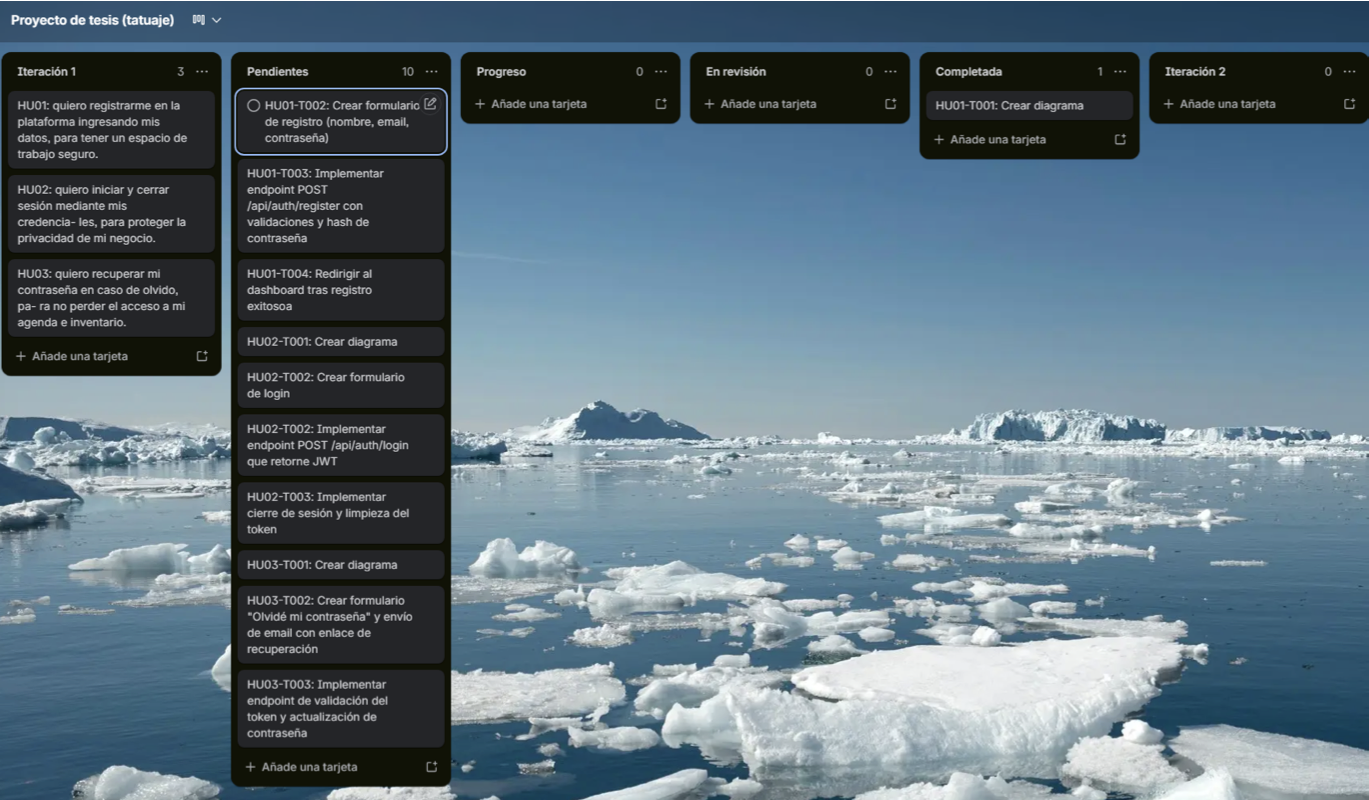
\includegraphics[width=0.8\textwidth]{fig-3-1-trello}
  \caption[Trello]{Extracto de la tabla dee registro de tareas por iteración.}
  \label{fig:trello}
\end{figure}

\titulopar{Diseño}

En esta etapa, se crean los diagramas de sencuencia de las historias de usuario asociadas a la iteración. A continuación, la Figura \ref{fig:secuencia} representa un ejemplo de diagrama de secuencia para el inicio de sesión.

\begin{figure}[H]
  \centering
  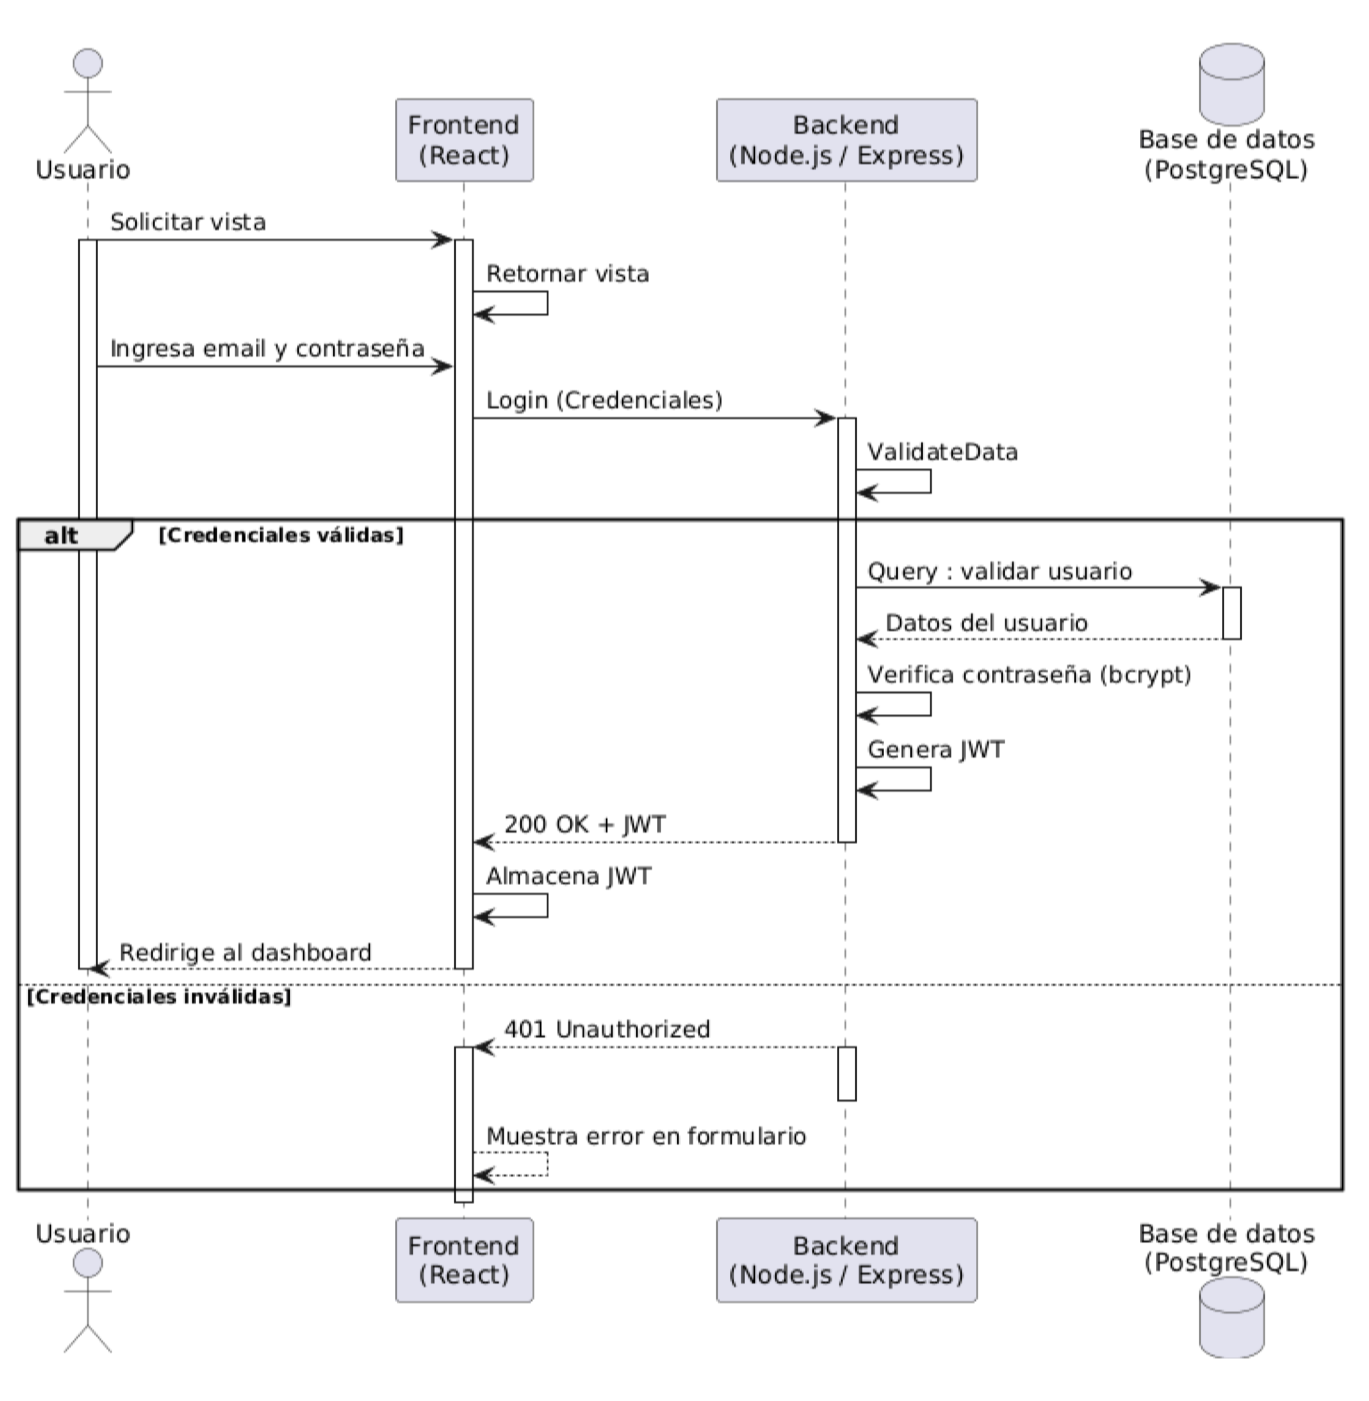
\includegraphics[width=0.8\textwidth]{fig-3-2-diagrama-secuencia}
  \caption[Diagrama de secuencia]{Ejemplo de diagrama de secuencia para el inicio de sesión.}
  \label{fig:secuencia}
\end{figure}

\titulopar{Implementación}

En esta etapa se lleva a cabo el desarrollo de código, pruebas unitarias y refactorización. La implementación sigue los diagramas de secuencia para guiar el flujo de las funcionalidades y los mockups propuestos. Aunque la metodología PXP sugiere un enfoque de Test-Driven Development (TDD)\cite{beck2002}, en el que primero se crean las pruebas, luego el código, y finalmente se realiza la refactorización este caso se ajustaría el proceso: primero se desarrollará el código, luego se completarán las pruebas unitarias, y se refactorizará en caso de que alguna prueba falle.

\titulopar{Sistema de pruebas}

En esta etapa se crean y ejecutan las pruebas correspondientes a todas las tareas definidas en el Inicio de Iteración. Si alguna de las pruebas falla, se regresa a la etapa de Implementación para realizar la refactorización necesaria y asegurar que el código cumpla con los requisitos definidos en las historias de usuario. Para llevar el control de las pruebas se utiliza una lista de verifiación en el mismo Trello a cada tarea, en donde se marcan las pruebas que han sido superadas y las que aún están pendientes o han fallado.

A continuación la Figura \ref{fig:checklist} muestra un ejemplo de una lista de verificación para una iteración en particular.

\begin{figure}[H]
  \centering
  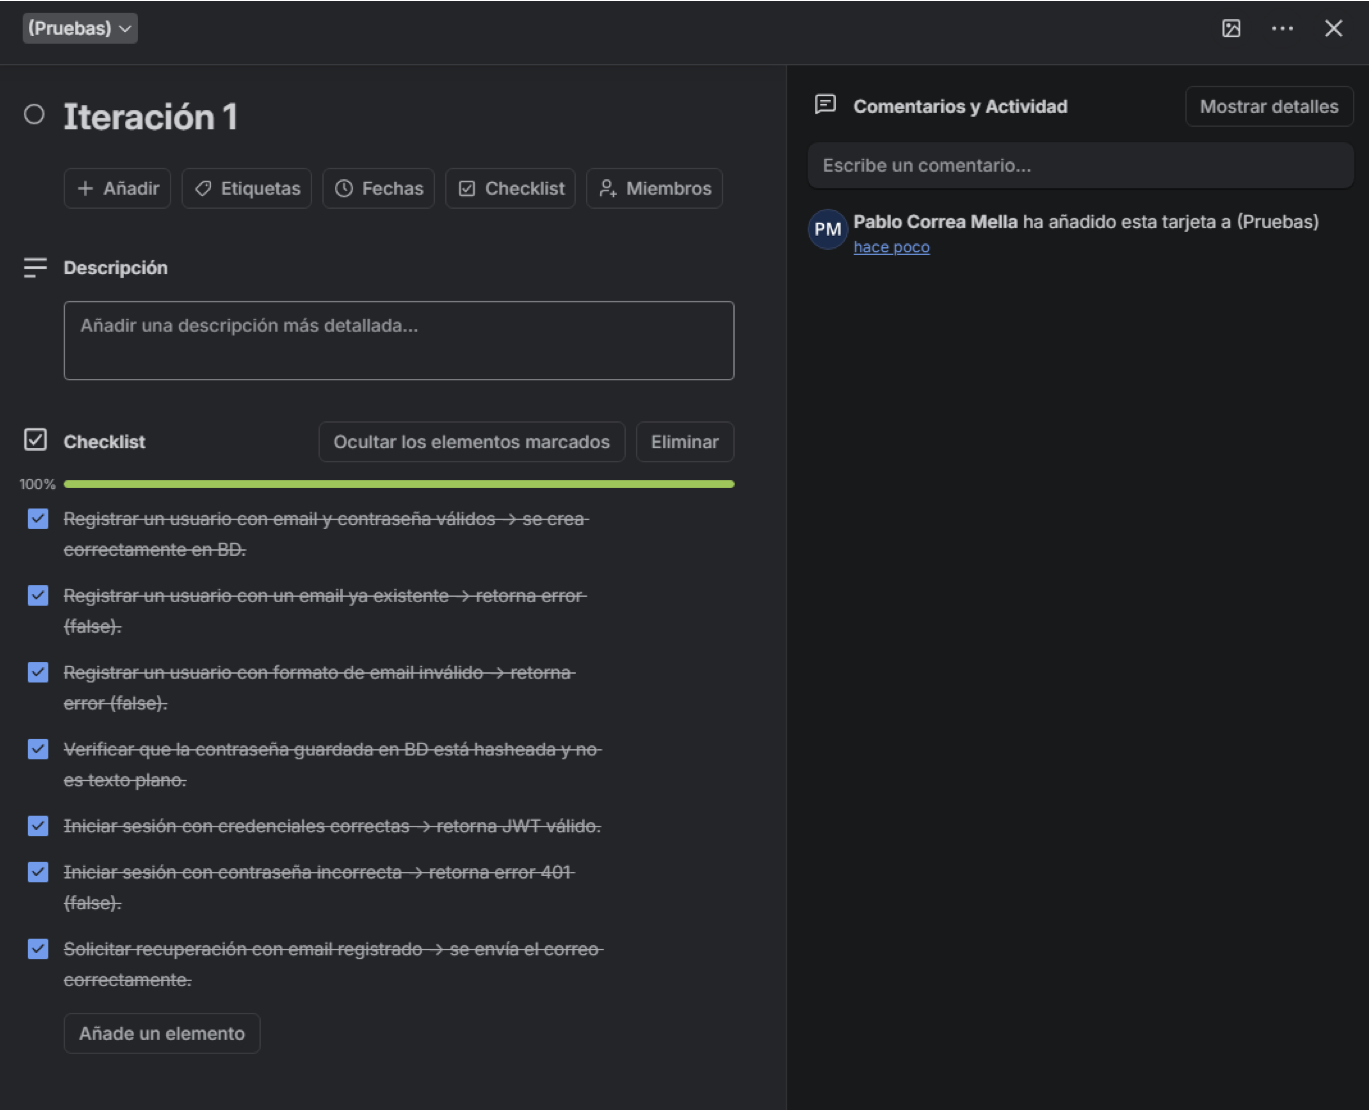
\includegraphics[width=0.8\textwidth]{fig-3-3-lista-verificacion}
  \caption[Lista de verificación de pruebas]{Ejemplo de lista de verificación de pruebas para una iteración.}
  \label{fig:checklist}
\end{figure}

\titulopar{Retrospectiva}

En esta etapa se realiza un análisis del desempeño del desarrollo, se integran las recomendaciones o ajustes detectados por el usuario experto, y se planifica el inicio de la siguiente iteración o el cierre definitivo del proyecto. Para llevar un control de las recomendaciones y ajustes, se utiliza una sección específica en Trello donde se documentan los comentarios recibidos durante la fase de pruebas, así como las acciones a tomar para mejorar el sistema en la siguiente iteración.

\section{Evaluación}

Como se mencionó en el Capítulo 2.5.2 para eevaluar el cumplimiento el objetivo general y los objetivos específicos, se implementarán distintas metodologías de evaluación, las cuales se describen a continuación.

\subsection{Prueba de caja negra}

Las pruebas de caja negra se enfocan en evaluar el funcionamiento de los módulos del sistema sin necesidad de conocer su proceso interno. En estas pruebas, se definen entradas específicas (por ejemplo, subir un boceto y asignar horas) y se comparan con las salidas esperadas en la interfaz de usuario, garantizando que los módulos operen correctamente de extremo a extremo. Para llevar un control de las pruebas de caja negra, se registran en una hoja de cálculo donde se documentan los casos de prueba definidos, las entradas utilizadas, las salidas esperadas y los resultados obtenidos, permitiendo así un seguimiento detallado del proceso de validación. A continuación, la Figura \ref{fig:registrocajanegra} muestra un ejemplo de cómo se registra una prueba de caja negra en la hoja de cálculo.

\begin{figure}[H]
  \centering
  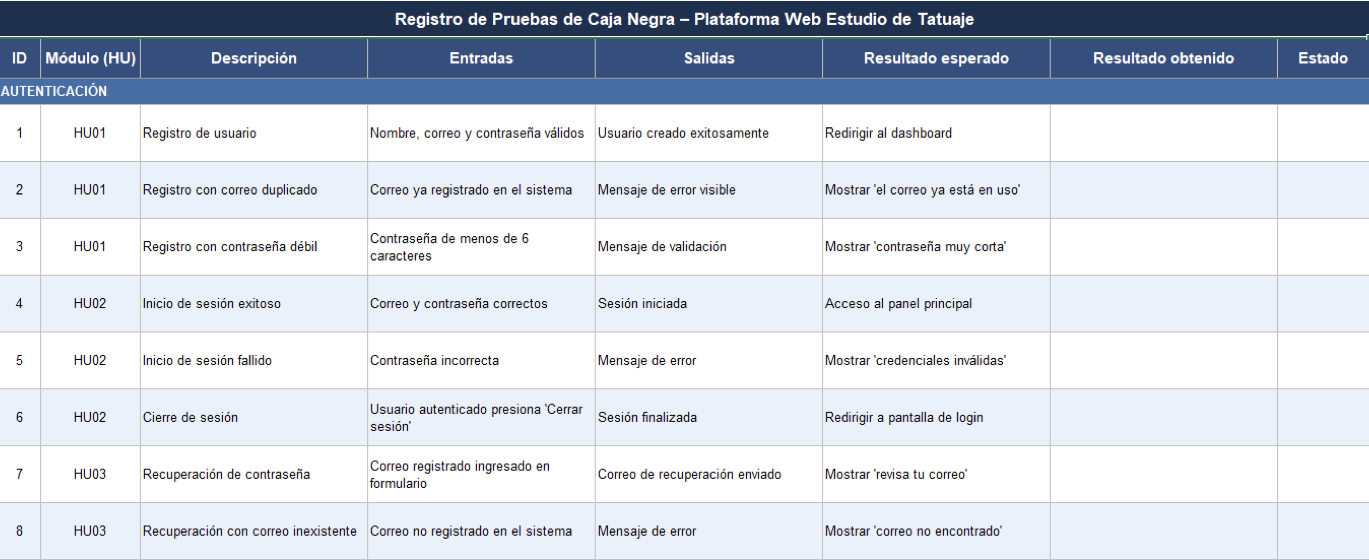
\includegraphics[width=0.8\textwidth]{fig-3-4-registro-caja-negra}
  \caption[Registro de prueba de caja negra]{Ejemplo de registro de prueba de caja negra en una hoja de cálculo.}
  \label{fig:registrocajanegra}
\end{figure}

\vspace{\parskip}
\subsection{Prueba de caja blanca }

Las pruebas de caja blanca se enfocan en verificar la lógica interna del código fuente, evaluando que los algoritmos críticos (como el motor de cálculo de cotizaciones y la lógica de proyección 3D) funcionen correctamente desde su interior. Se definen tests con el objetivo de alcanzar una cobertura de código de al menos un 95 \%. Para llevar un control de las pruebas de caja blanca, se utilizan herramientas de análisis de cobertura que generan reportes detallados sobre qué partes del código han sido ejecutadas durante las pruebas, permitiendo identificar áreas no cubiertas y asegurar que se cumpla con el objetivo establecido.

\subsection{Prueba de usabilidad}

La prueba de usabilidad SUS permite que el usuario final evalúe la aplicación mediante un cuestionario de 10 preguntas, que serán respondidas en una escala de Likert, con el objetivo de obtener una puntuación global que refleje la usabilidad del sistema. Para este proyecto, se ha establecido como métrica de éxito alcanzar un puntaje mínimo de 85 puntos, lo que indicaría que la plataforma es altamente usable y cumple con las expectativas del cliente experto. A continuación, se detallan las preguntas:

\vspace{\parskip}
\begin{enumerate}
  \item Creo que me gustaría usar esta plataforma con frecuencia.\\
  \item Encontré la plataforma innecesariamente compleja.\\
  \item Creo que la plataforma es fácil de usar.\\
  \item Creo que necesitaría la ayuda de una persona con conocimientos técnicos para usar esta plataforma.\\
  \item Creo que las funciones de esta plataforma están bien integradas.\\
  \item Creo que hay demasiada inconsistencia en esta plataforma.\\
  \item Imagino que la mayoría de las personas aprenderían a usar esta plataforma muy rápidamente.\\
  \item Creo que esta plataforma es muy difícil de usar.\\
  \item Creo que me sentiría muy seguro usando esta plataforma.\\
  \item Necesitaría aprender muchas cosas antes de poder usar esta plataforma.\\
\end{enumerate}
\vspace{\parskip}

Para obtener el grado de aceptación de la aplicación se debe realizar el siguiente cálculo:

\begin{itemize}
  \item Sumar las puntuaciones de las preguntas impares (1, 3, 5, 7, 9) y restar 5 al resultado.
  \item Sumar las puntuaciones de las preguntas pares (2, 4, 6, 8, 10) y restar el resultado a 25.
  \item Sumar los resultados de ambos cálculos y multiplicar por 2.5 para obtener la puntuación final en una escala de 0 a 100.
\end{itemize}
\vspace{\parskip}

El puntaje final, que varía entre 0 y 100, permite clasificar la usabilidad de la plataforma como Inaceptable (0-49), Mediocre (50-68) o Aceptable (69-100).

\subsection{Encuesta}

Este método de evaluación, como se detalla en el Capítulo 2.5.2, permite medir objetivos específicos comparando el estado inicial y final de las métricas evaluadas. Las preguntas de la encuesta están diseñadas para obtener respuestas númericas, lo que facilita la comparación de ambos estasdos. A continuación, se presentan algunas de las preguntas, en este caso las que se utilizan para determinar el estado inicial de los objetivos específicos.

\vspace{\parskip}
\begin{enumerate}
  \item ¿Cuánto tiempo promedio dedicas a ajustar o posicionar un boceto en papel para que se adapte a la curvatura de la piel? (en minutos)\\
  \item ¿Cuánto tiempo promedio dedicas a calcular el costo de un tatuaje manualmente? (en minutos)\\
  \item ¿Cuál es tu tasa de inasistencia semanal promedio? (en porcentaje)\\
  \item ¿Cuánto tiempo promedio dedicas a gestionar tu agenda y enviar recordatorios a tus clientes? (en minutos)\\
  \item ¿Cuánto tiempo promedio dedicas a organizar tu inventario y calcular el costo de los insumos? (en minutos)\\
  \mbox{}\\[-1.01pt]
\end{enumerate}

\section{Resultados esperados}

A continuación, se detallan los resultados esperados para cada uno de los objetivos específicos planteados en el Capítulo 1.2.2:

\begin{itemize}
  \item \textbf{Reducción del ausentismo (Objetivo Específico 2):}
  \begin{itemize}
    \item Resultado esperado: Se espera lograr una reducción del 50 \% en la tasa de inasistencia semanal al implementar el módulo de agendamiento con recordatorios automáticos por WhatsApp, en comparación con la tasa actual sin este sistema.
    \item Pruebas para lograr resultado esperado: Prueba de que el funcionamiento del módulo de agendamiento y recordatorios automáticos por WhatsApp realice el envío correcto de los mensajes 24 horas antes de la sesión programada, y que el cliente reciba estos mensajes sin fallos.
  \end{itemize}
  \item \textbf{Reducción del tiempo de cotización (Objetivo Específico 3):}
  \begin{itemize}
    \item Resultado esperado: Se espera lograr una reducción del 40 \% en los tiempos de cotización al utilizar el módulo de inventario y cálculo automatizado, en comparación con el método manual de cálculo.
    \item Pruebas para lograr resultado esperado: Prueba de que el funcionamiento del módulo de inventario y cálculo automatizado permita calcular los costos de manera precisa y rápida, en comparación con el método manual.
  \end{itemize}
  \item \textbf{Reducción del tiempo de previsualización (Objetivo Específico 4):}
  \begin{itemize}
    \item Resultado esperado:Se espera lograr una reducción del 30 \% en los tiempos de previsualización al utilizar el módulo de proyección 3D, en comparación con el método tradicional de ajuste manual en papel.
    \item Pruebas para lograr resultado esperado: Prueba de que el funcionamiento del módulo de proyección 3D permita ajustar y posicionar los bocetos de manera rápida y precisa sobre el modelo anatómico, en comparación con el método manual en papel.
  \end{itemize}
\end{itemize}

\section{Resumen capítulo}

En este capítulo se presentó detallademente la forma en que se aplicará la metodología PXP en el proyecto. También, se explican las metodologías de evaluación, mediante pruebas de software y, pruebas cualititativas y cuantitativas, en donde se agregan ejemplos de estas. Finalmente, se mencionan los resultados esperados, los cuales responden a los objetivos específicos planteados en el Capítulo 1.2.2.

En el siguiente capítulo se detallará la implementación de la metodología de desarrollo, en donde se explicará el trabajo realizado en las iteraciones, siguiendo las etapas de inicio de iteración, diseño, implementación, sistema de pruebas y retrospectiva.
